\documentclass{article}
\usepackage{graphicx}
\usepackage{amsmath}
\usepackage{listings}
\usepackage{geometry}
\usepackage{physics}
\usepackage[utf8]{inputenc}


\geometry{
 a4paper,
 total={170mm,257mm},
 left=20mm,
 top=20mm,
 }

\title{Assignment 8: The Digital Fourier Transform}
\author{Jineeth N [EE20B051]}
\date{6th May ,2022}

\begin{document}

\maketitle

\section{Introduction}
This assignment is about DFT and how it is implemented in python using Numpy's FFT module. We also attempt to approximate the continuous time fourier transform of a gaussian by windowing and sampling in time domain, and then taking the DFT.

\section{Tasks}
\subsection{FFT and IFFT}
We find the Fourier transform and invert it back to the time domain for a random signal, find maximum error to test the reconstruction

\begin{verbatim}
    # FFT of random values
    x = np.random.rand(100)
    X = fft(x)
    y = ifft(X)
    np.c_[x, y]
    print(abs(x - y).max())
\end{verbatim}

\subsection{Spectrum of sin(5t)}
The phase for some values near the peaks is non zero. To fix this we sample the input signal at an appropriate frequency. We also shift the phase plot so that it goes from $-\pi$ to $\pi$.

\begin{verbatim}
    # 1.) Calculating the DFT(Digital Fourier Transform) of sin(5t)
    x = np.linspace(0, 2*pi, 129); x = x[:-1]
    y = np.sin(5*x)
    Y0 = fftshift(fft(y))/128.0
    w0 = np.linspace(-64, 63, 128)
    
    plt.figure(0)
    
    # Magnitude Plot
    plt.subplot(2, 1, 1) # To plot magnitude and phase plot above and below at same pop up graph 
    plt.plot(w0, abs(Y0), lw = 2) # Magnitude plot
    plt.xlim([-10, 10]) # x(i.e., w{omega}) - axis limit 
    plt.ylabel("|Y|", size = 16)
    plt.title("Spectrum of sin(5t)")
    plt.grid(True)
    
    # Phase plot
    plt.subplot(2, 1, 2)
    plt.plot(w0, np.angle(Y0), 'ro', lw = 2) # Phase plot for all w 
    ii = np.where(abs(Y0) > 1e-3)
    plt.plot(w0[ii], np.angle(Y0[ii]), 'go', lw = 2) # Phase plot for such 'w' for which |Y| > 0.001
    plt.xlim([-10, 10])
    plt.ylabel("Phase of Y", size = 16)
    plt.xlabel("k", size = 16)
    plt.grid(True)
\end{verbatim}

\begin{figure}[!ht]
  \centering
  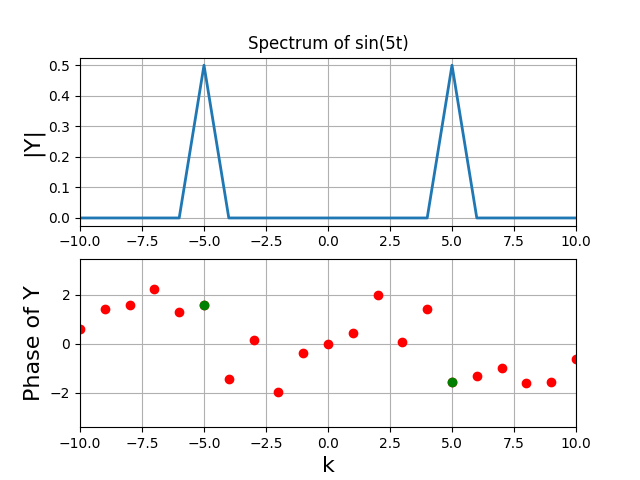
\includegraphics[scale=1]{Figure_0.png}
  \caption{Magnitude and Phase Plot of sin(5t)}
  \label{fig:sample}
  \end{figure}
As expected we get 2 peaks at +5 and -5 with height 0.5

\subsubsection{Amplitude Modulation}
Consider the signal:\newline
\begin{equation}
f(t) = (1+0.1\cos(t))\cos(10t)    
\end{equation}

We  expect  a  shifted  set  of  spikes,  with  a  main  impulse  and  two  side impulses on each side.  This is because,
\begin{equation}
    0.1cos(10t)cos(t) = 0.05(cos11t+cos9t)= 0.025(e11tj+e9tj+e11tj+e9tj)
\end{equation}

The Python code to calculate the DFT for above function is as follows:

\begin{verbatim}
   t1 = np.linspace(-4*pi, 4*pi, 513); t1 = t1[:-1] 
    y1 = (1 + 0.1*np.cos(t1))*np.cos(10*t1) 
    Y1 = fftshift(fft(y1))/512.0  
    w1 = np.linspace(-64,64,513); w1 = w1[:-1]
    
    plt.figure(1)
    
    
    # Magnitude Plot
    plt.subplot(2, 1, 1)
    plt.plot(w1, abs(Y1), lw = 2)
    plt.xlim([-15, 15])
    plt.ylabel("|Y|", size = 16)
    plt.title("Spectrum of (1 + 0.1cos(t))cos(10t)")
    plt.grid(True)
    
    # Phase plot 
    plt.subplot(2, 1, 2)
    plt.plot(w1, np.angle(Y1), 'ro', lw = 2)
    plt.xlim([-15, 15])
    plt.ylabel("Phase of Y", size = 16)
    plt.xlabel("ω", size = 16)
    plt.grid(True)

\end{verbatim}

\begin{figure}[!ht]
  \centering
  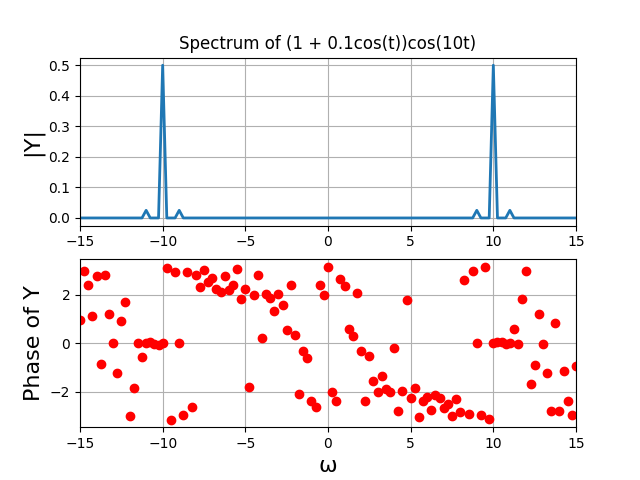
\includegraphics[scale=1]{Figure_1.png}
      \caption{Magnitude and Phase Plot of (1 + 0.1cos(t))*cos(10t)}
      \label{fig:sample}
      \end{figure}

\subsubsection{Spectrum of $sin^3(t)$}
This signal can be expressed as a sum of sine waves using this identity:\newline
\begin{equation}
   \sin^3(t) = \frac{3}{4}\sin(t) - \frac{1}{4}\sin(3t) 
\end{equation}

The Python code for above function is as follows:
\begin{verbatim}
    t3 = np.linspace(-4*pi, 4*pi, 513); t3 = t3[:-1]
    y3 = (np.sin(t3))**3
    Y3 = fftshift(fft(y3))/512.0
    w3 = np.linspace(-64, 64, 513); w3 = w3[:-1]
    
    plt.figure(3)
    
    # Magnitude Plot
    plt.subplot(2, 1, 1)
    plt.plot(w3, abs(Y3), lw = 2)
    plt.xlim([-15, 15])
    plt.ylabel("|Y|", size = 16)
    plt.title("Spectrum of sin\u00B3(t)")
    plt.grid(True)
    
    # Phase Plot
    plt.subplot(2, 1, 2)
    plt.plot(w3, np.angle(Y3), 'ro', lw = 2)
    plt.xlim([-15, 15])
    plt.ylabel("Phase of Y", size = 16)
    plt.xlabel("ω", size = 16)
    plt.grid(True)

\end{verbatim}

\begin{figure}[!ht]
  \centering
  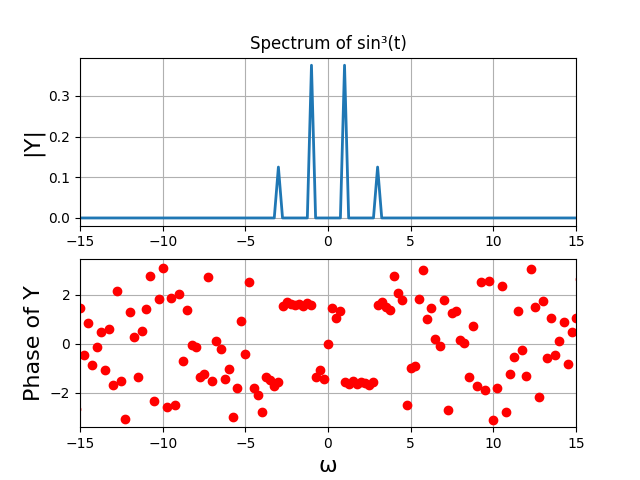
\includegraphics[scale=1]{Figure_3.png}
  \caption{Magnitude Plot of $sin^3(t)$}
  \label{fig:sample}
  \end{figure}
  
\subsubsection{Spectrum of $cos^3(t)$}
This signal can be expressed as a sum of cosine waves using this identity:
\begin{equation}
    sin^3(t) = \frac{3}{4}\cos(t) + \frac{1}{4}\cos(3t)
\end{equation}

The Python code for above function is as follows:
\begin{verbatim}
    t2 = np.linspace(-4*pi, 4*pi, 513); t2 = t2[:-1]
    y2 = (np.cos(t2))**3
    Y2 = fftshift(fft(y2))/512.0
    w2 = np.linspace(-64, 64, 513); w2 = w2[:-1]
    
    
    # Magnitude plot
    plt.figure(2)
    plt.subplot(2, 1, 1)
    plt.plot(w2, abs(Y2), lw = 2)
    plt.xlim([-15, 15])
    plt.ylabel("|Y|", size = 16)
    plt.title("Spectrum of cos\u00B3(t)")
    plt.grid(True)
    
    # Phase plot
    plt.subplot(2, 1, 2)
    plt.plot(w2, np.angle(Y2), 'ro', lw = 2)
    plt.xlim([-15, 15])
    plt.ylabel("Phase of Y", size = 16)
    plt.xlabel("ω",size = 16)
    plt.grid(True)
\end{verbatim}

\begin{figure}[!ht]
  \centering
  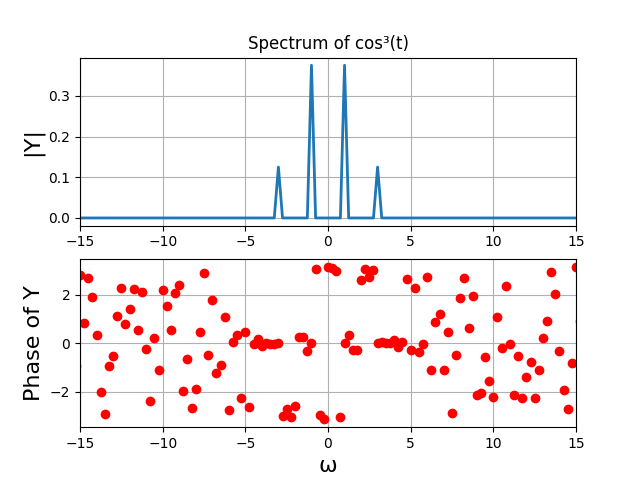
\includegraphics[scale=1]{Figure_2.png}
  \caption{Magnitude Plot of $cos^3(t)$}
  \label{fig:sample}
  \end{figure}

\subsection{Spectrum of frequency Modulated wave}
Consider the signal:\newline
\begin{equation}
f(t) =  \cos(20t +5 \cos(t))    
\end{equation}

The Python code for above function is as follows:

\begin{verbatim}
    t4 = np.linspace(-4*pi, 4*pi, 513); t4 = t4[:-1]
    y4 = np.cos(20*t4 + 5*np.cos(t4))
    Y4 = fftshift(fft(y4))/512.0
    w4 = np.linspace(-64, 64, 513); w4 = w4[:-1]
    
    plt.figure(1)
    
    # Magnitude Plot
    plt.subplot(2, 1, 1)
    plt.plot(w4, abs(Y4), lw = 2)
    plt.xlim([-30, 30])
    plt.ylabel("|Y|", size = 16)
    plt.title("Spectrum of cos(20t + 5cos(t))")
    plt.grid(True)
    
    # Phase Plot
    plt.subplot(2, 1, 2)
    ii = np.where(abs(Y4) > 1e-3)
    plt.plot(w4[ii], np.angle(Y4[ii]), 'go', lw = 2)
    plt.xlim([-30, 30])
    plt.ylabel("Phase of Y", size = 16)
    plt.xlabel("ω", size = 16)
    plt.grid(True)

\end{verbatim}

\begin{figure}[!ht]
  \centering
  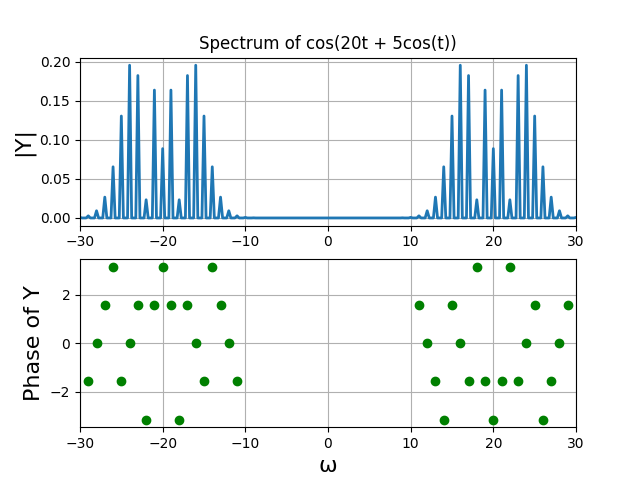
\includegraphics[scale=1]{Figure_1.1.png}
  \caption{Magnitude Plot of $cos(20t +5 cos(t))$}
  \label{fig:sample}
  \end{figure}

\subsection{Spectrum of Gaussian Function}
The Fourier transform of a signal $x(t)$ is defined as follows:\newline
\begin{equation}
X(\omega) = \frac{1}{2 \pi} \int_{- \infty}^{\infty} x(t) e^{-j \omega t} dt   
\end{equation}
As Gaussian Function tends to $0$ for large values of $t$, we can approximate the above equation as shown below. And the appropriate values of T will be calculated using iterations
\begin{equation}
  X(\omega) \approx \frac{1}{2 \pi} \int_{- T/2}^{T/2} x(t) e^{-j \omega t} dt  
\end{equation}
The expression for the Gaussian is :
\begin{equation}
    x(t) = e^{\frac{-t^2}{2}}    
\end{equation}
The CTFT is given by:
\begin{equation}
X(j \omega) = \frac{1}{\sqrt{2 \pi}}e^{\frac{-\omega^2}{2}}    
\end{equation}

\begin{verbatim}
The Python code for above function is as follows:

    def gaussFn(x):
    return np.exp(-0.5*x**2)

def ExpectedGauss(w):
    return 1/np.sqrt(2*pi) * np.exp(-w**2/2)

def estdft(tolerance = 1e-6, samples = 128, func = gaussFn, expectedfn = ExpectedGauss, wlim = 5):
    T = 8*pi
    N = samples
    Yold = 0
    error = tolerance + 1
    iter = 0
    # Iterative loop to find window size
    while error > tolerance:  
        x = np.linspace(-T/2, T/2, N + 1)[:-1]
        w = np.linspace(-N*pi/T, N*pi/T, N + 1)[:-1]
        y = gaussFn(x)
        Y = fftshift(fft(fftshift(y)))*T/(2*pi*N)
        error = sum(abs(Y[::2] - Yold))
        Yold = Y
        iter += 1
        T *= 2
        N *= 2
        

    # Calculating error
    true_error = sum(abs(Y - expectedfn(w))) # Absolute error
    print("True error: ", true_error)
    print("Samples = " + str(N))
    print("Time period = " + str(T))

    mag = abs(Y)
    phi = np.angle(Y)
    phi[np.where(mag < tolerance)] = 0
    
    ######
    # 6.) Plotting estimated output
    plt.figure()
    
    # Magnitude Plot
    plt.subplot(2, 1, 1)
    plt.plot(w, abs(Y), lw = 2)
    plt.xlim([-wlim, wlim])
    plt.ylabel('Magnitude', size = 16)
    plt.title("Estimated FFT of Gaussian")
    plt.grid(True)

    # Phase Plot
    plt.subplot(2, 1, 2)
    plt.plot(w, np.angle(Y), 'ro', lw = 2)
    ii = np.where(abs(Y) > 1e-3)
    plt.plot(w[ii], np.angle(Y[ii]), 'go', lw = 2)
    plt.xlim([-wlim, wlim])
    plt.ylabel("Phase", size = 16)
    plt.xlabel("ω", size = 16)
    plt.grid(True)
    

    #######
    # 7.) Plotting expected output    
    Y_out = expectedfn(w)
    
    mag = abs(Y_out)
    phi = np.angle(Y_out)
    phi[np.where(mag < tolerance)] = 0
    
    plt.figure()
    
    # Magnitude Plot
    plt.subplot(2, 1, 1)
    plt.plot(w, abs(Y), lw = 2)
    plt.xlim([-wlim, wlim])
    plt.ylabel('Magnitude', size = 16)
    plt.title("True FFT of Gaussian")
    plt.grid(True)

    # Phase Plot
    plt.subplot(2, 1, 2)
    plt.plot(w, np.angle(Y), 'ro', lw = 2)
    ii = np.where(abs(Y) > 1e-3)
    plt.plot(w[ii], np.angle(Y[ii]), 'go', lw = 2)
    plt.xlim([-wlim, wlim])
    plt.ylabel("Phase", size = 16)
    plt.xlabel("ω",size = 16)
    plt.grid(True)
   
\end{verbatim}

\begin{figure}[!ht]
  \centering
  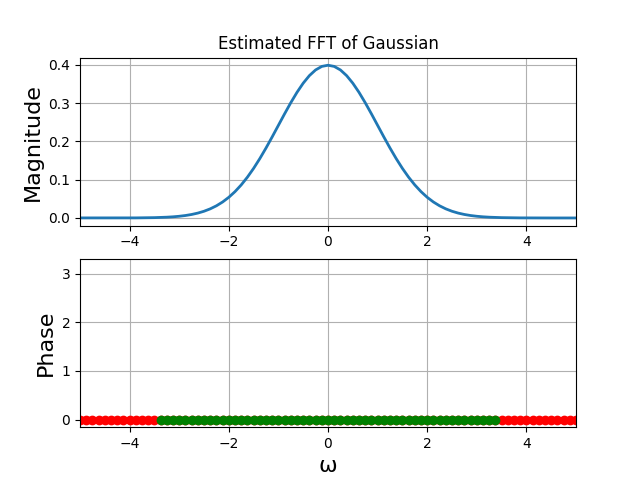
\includegraphics[scale=1]{Figure_1.2.png}
  \caption{Magnitude Plot of $e^{\frac{-t^2}{2}}$}
  \label{fig:sample}
  \end{figure}

\newpage
\section{Conclusion}
We analysed the Discrete Fourier Transforms of sinusoids, amplitude and frequency modulated signals using FFT library in python. The pure sinusoids contained impulses at given frequncies. The frequency modulated wave contains many frequencies. Also we verified that DFT of a gaussian is gaussian function in $w$
                                                        
\end{document}
